\begin{tikzpicture}

%A matrix
\draw [fill=cyan, opacity=.2,rotate=90, thick]  (0.1,5.6) node (v1) {} rectangle (3.9,-1.4) node (v2) {};
\draw [thick,rotate=90,red] (v1) rectangle (3.9,4.6);
\draw [thick,rotate=90,red] (0.1,4.6) rectangle (3.9,3.6) node (v7) {};
\draw [thick,rotate=90,red] (0.1,-0.4) node (v6) {} rectangle (v2);
\draw[thick,red]  (v6) rectangle (-0.6,3.9);
\draw[thick,red]  (v7) rectangle (-2.6,0.1);

\node at (-6.2,1.6) { \color{blue}\Large  \bf  \vdots};
\node  at (-6.2,3.6) {\color{blue} \bf  \Large $\underline{a_1}$};
\node at (-6.2,2.6) { \color{blue} \bf  \Large $\underline{a_2}$};
\node at (-6.2,0.6) {\color{blue} \bf  \Large $\underline{a_m}$};
\node at (-2.2,-1.4) {\huge$ \underset{ \color{blue} ( m \ll n)}{A_{ m \times n} }$};

% X vector
\draw [ thick, fill=green] (4,5) rectangle (5,6);
\draw [thick] (5,5) rectangle (4,4);
\draw [thick, fill=green] (4,4) rectangle (5,3);
\draw [] (4,3) node (v4) {} rectangle (5,-0.1) node (v5) {};
\draw [thick] (4,-0.1) rectangle (5,-1.1);
\draw [thick, fill=green] (4,-1.1) rectangle (5,-2.1);
\node at (4.6,-3.4) {\huge $\underset{\tiny \color{blue} (K-sparse)}{x_{n \times 1 }} $};
\node at (4.5,1.6) {\Large \bf \vdots};
\node at (2.7,2.1) {\Huge $\times$};
\draw [thick] (v4) rectangle (5,2.1);
\draw [thick] (v5) rectangle (4,0.8);

% y

\draw [thick] (-10.3,4.1) node (v3) {} rectangle (-9.3,3.1);
\draw [thick] (-10.3,3.1) rectangle (-9.3,2.1);
\draw [thick] (-10.3,2.1) rectangle (-9.3,1);
\draw [thick] (-10.3,1) rectangle (-9.3,0);
\draw[fill=red, opacity=0.2]  (v3) rectangle (-9.3,0);
\node at (-3.1,1.6) { \color{blue}\Large  \bf  \vdots};


\node at (-9.8,1.6) {\bf \vdots};

\node at (-7.7,2) {\Huge = };
\node at (-9.7,-1.2) {\huge $ \underset{ \color{blue} (Observations) }{y_{m \times 1}}$};


\node at (-1.6,2.5) {\Huge \color{red} \bf $\cdots$};
\draw [dashed,blue] (-5.6,3.9) rectangle (1.4,3);
\draw [dashed,blue] (-5.6,3) rectangle (1.4,2);
\draw[dashed,blue]  (v1) rectangle (1.4,1);
\node at (-5.15,4.5) {\Large \bf  \color{red} $b_0$};
\node at (-4,4.5) {\Large \bf \color{red} $b_1$};
\node at (-3,4.5) {\Large \bf  \color{red} $b_2$};
\node at (-1.5,4.5) {\Large \bf  \color{red} $\cdots$};
\node at (0,4.5) {\Large \bf  \color{red} $b_{n-1}$};
\node at (1,4.5) {\Large \bf  \color{red} $b_n$};
\end{tikzpicture}